\documentclass[
  bibliography=totoc,     % Literatur im Inhaltsverzeichnis
  captions=tableheading,  % Tabellenüberschriften
  titlepage=firstiscover,
  fontsize=12pt, % Titelseite ist Deckblatt
]{scrartcl}

% Paket float verbessern
\usepackage{scrhack}

% Warnung, falls nochmal kompiliert werden muss
\usepackage[aux]{rerunfilecheck}

% unverzichtbare Mathe-Befehle
\usepackage{amsmath}
% viele Mathe-Symbole
\usepackage{amssymb}
% Erweiterungen für amsmath
\usepackage{mathtools}

% Fonteinstellungen
\usepackage{fontspec}
\setmainfont{Arial}
% Wenn man andere Schriftarten gesetzt hat,
% sollte man das Seiten-Layout neu berechnen lassen
\recalctypearea{}

% deutsche Spracheinstellungen
\usepackage[british]{babel}

\usepackage[
  math-style=ISO,    % ┐
  bold-style=ISO,    % │
  sans-style=italic, % │ ISO-Standard folgen
  nabla=upright,     % │
  partial=upright,   % ┘
  warnings-off={           % ┐
    mathtools-colon,       % │ unnötige Warnungen ausschalten
    mathtools-overbracket, % │
  },                       % ┘
]{unicode-math}

% traditionelle Fonts für Mathematik
\setmathfont{Latin Modern Math}
% Alternativ zum Beispiel:
% \setmathfont{Libertinus Math}

\setmathfont{XITS Math}[range={scr, bfscr}]
\setmathfont{XITS Math}[range={cal, bfcal}, StylisticSet=1]

% Zahlen und Einheiten
\usepackage[
  locale=UK,                   % deutsche Einstellungen
  separate-uncertainty=true,   % immer Unsicherheit mit \pm
  per-mode=symbol-or-fraction, % / in inline math, fraction in display math
]{siunitx}

% chemische Formeln
\usepackage[
  version=4,
  math-greek=default, % ┐ mit unicode-math zusammenarbeiten
  text-greek=default, % ┘
]{mhchem}

% richtige Anführungszeichen
\usepackage[autostyle]{csquotes}

% schöne Brüche im Text
\usepackage{xfrac}

% Standardplatzierung für Floats einstellen
\usepackage{float}
\floatplacement{figure}{htbp}
\floatplacement{table}{htbp}

% Floats innerhalb einer Section halten
\usepackage[
  section, % Floats innerhalb der Section halten
  below,   % unterhalb der Section aber auf der selben Seite ist ok
]{placeins}

% Seite drehen für breite Tabellen: landscape Umgebung
\usepackage{pdflscape}

% Captions schöner machen.
\usepackage[
  labelfont=bf,        % Tabelle x: Abbildung y: ist jetzt fett
  font=small,          % Schrift etwas kleiner als Dokument
  width=0.9\textwidth, % maximale Breite einer Caption schmaler
]{caption}
% subfigure, subtable, subref
\usepackage{subcaption}

% Grafiken können eingebunden werden
\usepackage{graphicx}

% schöne Tabellen
\usepackage{booktabs}

% Verbesserungen am Schriftbild
\usepackage{microtype}

% Literaturverzeichnis
\usepackage[
  backend=biber,
]{biblatex}
% Quellendatenbank
\addbibresource{lit.bib}
% \addbibresource{programme.bib}

% Hyperlinks im Dokument
\usepackage[
  german,
  unicode,        % Unicode in PDF-Attributen erlauben
  pdfusetitle,    % Titel, Autoren und Datum als PDF-Attribute
  pdfcreator={},  % ┐ PDF-Attribute säubern
  pdfproducer={}, % ┘
]{hyperref}
% erweiterte Bookmarks im PDF
\usepackage{bookmark}

% Trennung von Wörtern mit Strichen
\usepackage[shortcuts]{extdash}

\author{%
  Lennart Völz\\%
  \href{mailto:lennart.voelz@tu-dortmund.de}{lennart.voelz@tu-dortmund.de}%
  \and%
  Max Möller\\%
  \href{mailto:max2.moeller@tu-dortmund.de}{max2.moeller@tu-dortmund.de}%
}
\publishers{TU Dortmund – Fakultät Physik}

% Line spacing
\usepackage{setspace}
\onehalfspacing

% Margins
\usepackage[left=2.5cm, right=2.5cm, top=3.5cm, bottom=3.5cm]{geometry}

\usepackage{adjustbox}

% Allow line breaks
\sloppy


\begin{document}
%1
\maketitle
%2
\begin{frame}{\huge{Definition and motivation of problem task}}
  \begin{itemize}
    \item \textbf{Research question:} Can a computer vision algorithm truthfully detect driver inattention, using a convolutional neural network? 
    \item \textbf{Motivation:} Enhancing Road Safety: Driver inattention is a leading cause of road accidents. By detecting inattention early, potential collisions and accidents can be prevented, thereby saving lives and reducing injuries.
  \end{itemize}
\end{frame}
% 
\begin{frame}{\huge{Description of the Dataset}}
  \begin{columns}
    \column{.6\textwidth}
      \begin{itemize}
        \item \textbf{Source:} \url{https://universe.roboflow.com/driver-monitoring/dmd-tfiw0} provided by Roboflow user
        \item \textbf{License:} CC BY 4.0 - Freedom to Share and Adapt
        \item \textbf{Content of the Dataset:} Labeled pictures in .jpg format, displaying male drivers in different states of attention
        \item \textbf{Size of the Dataset:} 14859 pictures, (train: 80 \%, valid: 13 \%, test: 7 \%)
        \item \textbf{Input features:} Greyscale image
        \item \textbf{Classes:}
        \begin{itemize}
          \item[-] Dangerous driving - 4642 pictures
          \item[-] Distraction - 2080 pictures
          \item[-] Drinking - 428 pictures
          \item[-] Safe driving - 6180 pictures
          \item[-] Sleepy driving - 979 pictures
          \item[-] Yawn - 546 pictures
        \end{itemize}
      \end{itemize}
    \column{.4\textwidth}
      \begin{figure}
        \centering
        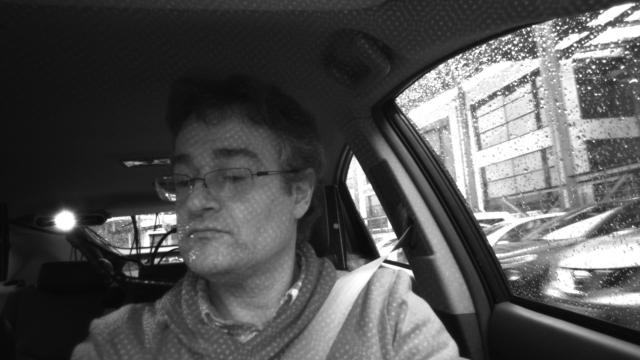
\includegraphics[width=\textwidth]{content/gA_1_s1_ir_face_mp4-26_jpg.rf.8073bccb5c613d34b8f058da71adc5d8.jpg}
        \caption{Example picture of the dataset.}
      \end{figure}
  \end{columns}
\end{frame}

\begin{frame}{\huge{Network architecture and method}}
  % \begin{columns}
    % \column{0.6\textwidth}
    \begin{figure}
      \centering
      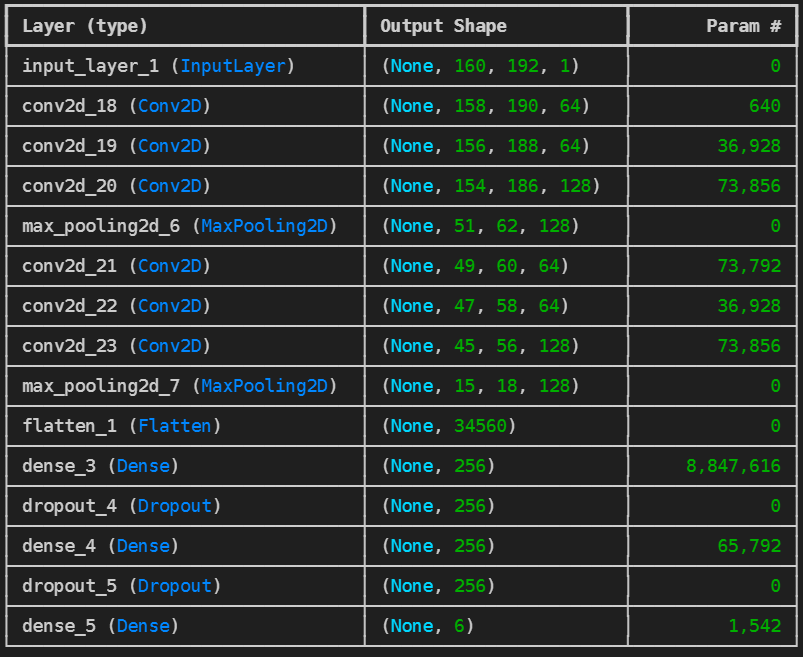
\includegraphics[width=.99\textheight]{content/arch.png}
      \caption{Network architecture of the convolutional neural network.}
    \end{figure}
\end{frame}

\begin{frame}{\huge{Network architecture and method}}
  \begin{table}[h!]
    \centering
    \begin{tabular}{>{\raggedright\arraybackslash}m{6cm} >{\raggedright\arraybackslash}m{6cm}}
    \toprule
    \textbf{Parameter} & \textbf{Value} \\
    \midrule
    Input Shape & \((192, 160, 1)\) \\
    Filters & 64 \\
    Kernel Size & \((3, 3)\) \\
    Pool Size & \((3, 3)\) \\
    Padding & valid \\
    Dropout Rate & 0.4 \\
    Optimizer & Adam (learning\_rate=0.0005) \\
    Loss Function & Categorical Crossentropy \\
    Metrics & Accuracy \\
    Early Stopping & val\_loss, Patience: 7 \\
    hidden layers activation & elu \\
    output layer activation & softmax \\
    \bottomrule
    \end{tabular}
    \caption{Model parameters used for training.}
    \label{table:parameters}
    \end{table}
\end{frame}

\begin{frame}{\huge{Optimization}}
  \begin{itemize}
    \item \textbf{Hyperparameter optimization:}
    \begin{itemize}
      \item[-] Not yet performed on current architecture, parameters taken from last iteration
      \item[-] Future work: Random search to constrain parameter space, Bayesian optimization to find optimal hyperparameters
    \end{itemize}
    \item \textbf{Regularization:}
    \begin{itemize}
      \item[-] Dropout layer
      % \item[-] Early stopping
      \item[-] L2 kernel regularization
      \item[-] Optimal parameters not yet known
    \end{itemize}
    \item \textbf{Class Inbalance:}
      \begin{itemize}
        \item[-] Created two alternative augmented datasets to balance classes
        \item[-] Future work: Compare performance of the different datasets
      \end{itemize}
    \item \textbf{Cross validation:} Datasets for the cross validation have been created
    \item \textbf{Other:} Implemented hard crop on all pictures to remove background noise
  \end{itemize}
\end{frame}

\begin{frame}{\huge{Results}}
  \begin{columns}
    \column{.5\textwidth}
    \begin{itemize}
      \item \textbf{Performance:}
      \begin{itemize}
        \item[-] Training accuracy: 0.9342
        \item[-] Validation accuracy: 0.8892
      \end{itemize}
      \item Trained non augmented dataset
      \item Automatically aborted after 35 epochs, due to early stopping
      \begin{itemize}
        \item[-] Currently overfitting
        \item[-] training accuracy not stagnating yet, leaves room for optimization
      \end{itemize}
    \end{itemize}
    \column{.5\textwidth}
      \begin{figure}
        \centering
        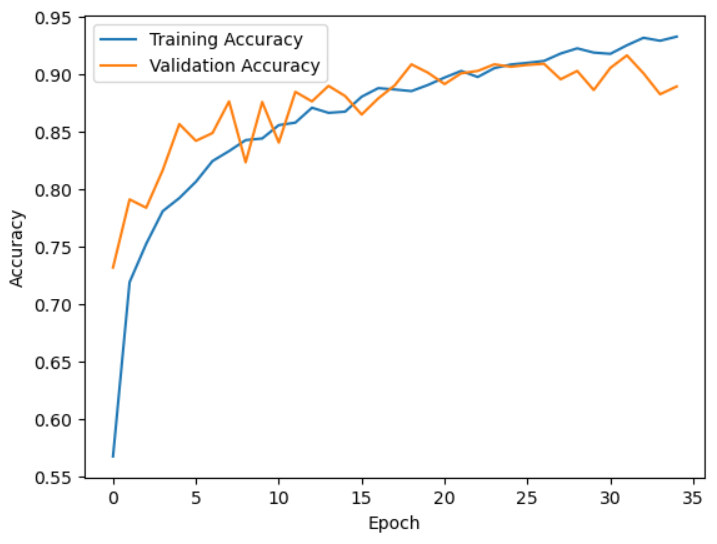
\includegraphics[width=\textwidth]{content/accuracy_plot.png}
        \caption{Plot of accuracy on training and validation data.}
      \end{figure}
  \end{columns}
\end{frame}

\begin{frame}{\huge{Comparison to alternative methods}}
  \begin{itemize}
    \item Comparison to the pretrained model, which is accessible through the website.
    \begin{itemize}
      \item[-] Previous work is general computer vision model not specific to the dataset
      \item[-] Use precision of pretrained model as comparison baseline 
    \end{itemize}
    \vspace{5mm}
    \begin{figure}[H]
      \centering
      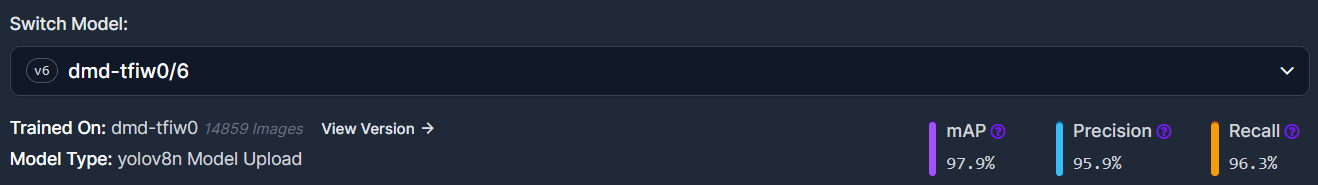
\includegraphics[width=.9\textwidth]{content/prec_pret.png}
      \caption{Precision of Roboflow interference model.}
    \end{figure}
  \end{itemize}
\end{frame}

\begin{frame}{\huge{Conclusion}}
  \begin{itemize}
    \item No conclusion can be made at the moment
    \item First results show already high accuracy with room for improvement
    \item Accuracy of Roboflow interference model might be matchable with good optimization
  \end{itemize}
\end{frame}

\end{document}